%% fig_quarticlocal.tex   (generated by make_round24.py; do not edit by hand)
%% The support of E' near a point of the glued curve, the two eigenplanes of the real multiplication at that point, and the table of nonzero products of translation classes for the ten germs of the computation (lem:freegerm, thm:quarticlocal, cor:markmanquarticfails).
\documentclass[tikz,border=8pt]{standalone}
\usepackage{amsmath,amssymb}
\usetikzlibrary{arrows.meta,calc,decorations.pathreplacing}
%% palette.tex -- shared colour definitions for the figures
\definecolor{PInk}{RGB}{26,32,44}
\definecolor{PBlue}{RGB}{37,82,139}
\definecolor{PTeal}{RGB}{23,127,125}
\definecolor{POchre}{RGB}{193,138,44}
\definecolor{PClay}{RGB}{178,74,58}
\definecolor{PSlate}{RGB}{108,122,137}
\definecolor{PViolet}{RGB}{110,86,150}
\definecolor{WBlue}{RGB}{223,234,246}
\definecolor{WTeal}{RGB}{220,238,236}
\definecolor{WOchre}{RGB}{250,240,218}
\definecolor{WClay}{RGB}{247,229,224}
\definecolor{WSlate}{RGB}{238,241,244}
\definecolor{PMag}{RGB}{158,58,110}
\definecolor{PGrass}{RGB}{62,124,66}
\definecolor{PAmber}{RGB}{214,112,38}
\definecolor{PIndigo}{RGB}{58,64,140}
\definecolor{PRule}{RGB}{176,186,197}

%% shared macros so the standalone figures match the paper
\providecommand{\QQ}{\mathbb{Q}}
\providecommand{\ZZ}{\mathbb{Z}}
\providecommand{\RR}{\mathbb{R}}
\providecommand{\CC}{\mathbb{C}}
\providecommand{\PP}{\mathbb{P}}
\providecommand{\Kx}{K^{\times}}
\providecommand{\HW}{W}
\providecommand{\Nm}{\mathrm{N}}
\providecommand{\Hdg}{\mathrm{Hdg}}
\providecommand{\NS}{\mathrm{NS}}
\providecommand{\cA}{\mathcal{A}}
\providecommand{\cD}{\mathcal{D}}
\providecommand{\cF}{\mathcal{F}}
\providecommand{\cP}{\mathcal{P}}
\providecommand{\cO}{\mathcal{O}}
\providecommand{\cQ}{\mathcal{Q}}
\providecommand{\bbar}[1]{\overline{#1}}
\providecommand{\ch}{\operatorname{ch}}
\providecommand{\End}{\mathrm{End}}
\providecommand{\Ext}{\operatorname{Ext}}
\providecommand{\Supp}{\operatorname{Supp}}

\begin{document}
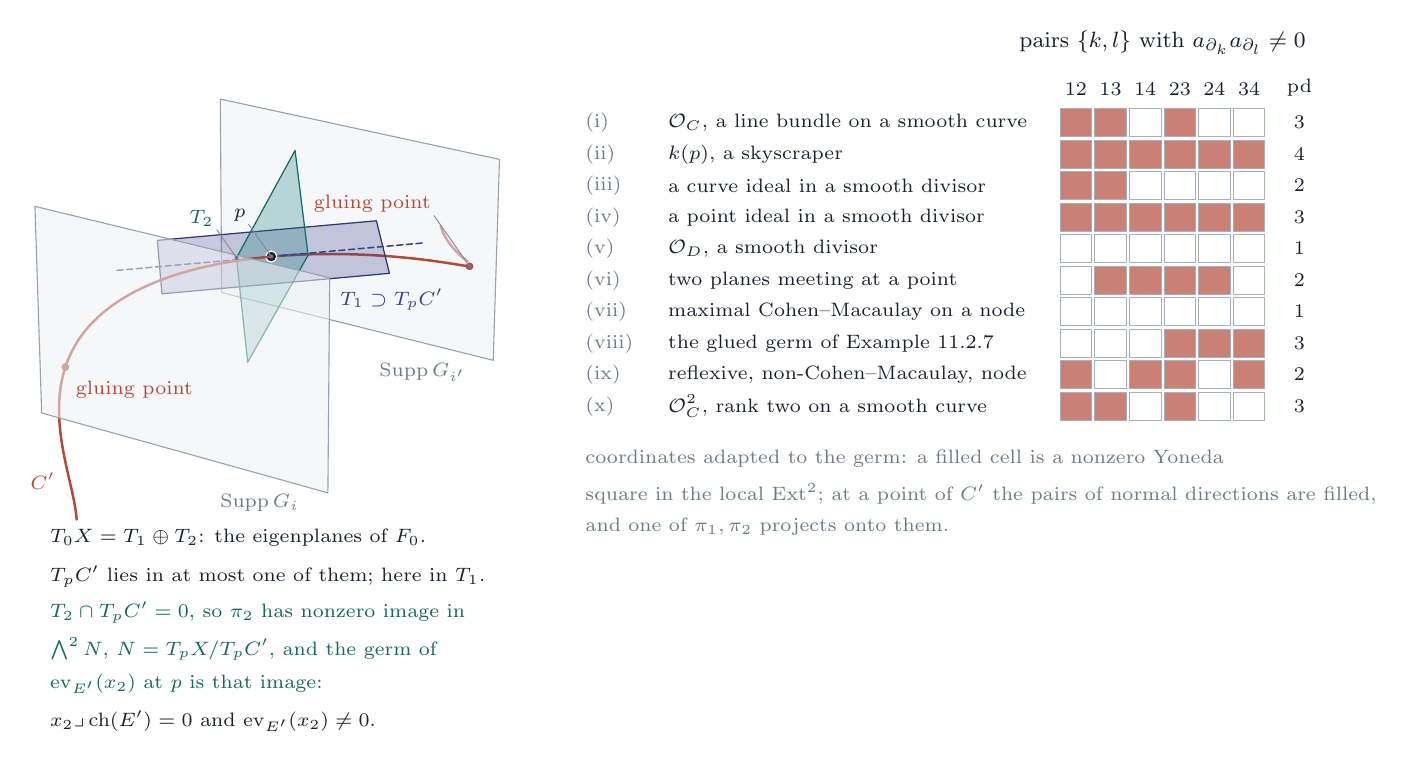
\begin{tikzpicture}[x=1cm,y=1cm,line join=round,line cap=round,
  font=\small,text=PInk,lbl/.style={inner sep=1pt}]
  \draw[PClay,line width=0.9pt] (2.2490,0.4334) -- (2.2338,0.4563) -- (2.2192,0.4799) -- (2.2055,0.5043) -- (2.1926,0.5294) -- (2.1808,0.5551) -- (2.1700,0.5815) -- (2.1604,0.6086) -- (2.1522,0.6363);
  \draw[PClay,line width=0.9pt] (2.3841,0.2785) -- (2.3670,0.2950) -- (2.3497,0.3123) -- (2.3324,0.3305) -- (2.3151,0.3495) -- (2.2981,0.3693) -- (2.2813,0.3899) -- (2.2649,0.4113) -- (2.2490,0.4334);
  \draw[PClay,line width=0.9pt] (2.5026,0.1768) -- (2.4906,0.1865) -- (2.4776,0.1971) -- (2.4637,0.2085) -- (2.4490,0.2208) -- (2.4335,0.2339) -- (2.4175,0.2479) -- (2.4010,0.2628) -- (2.3841,0.2785);
  \path[fill opacity=0.55,fill=WSlate,draw=PSlate!70,line width=0.40pt] (-0.6308,-0.2101) -- (2.8180,-1.0701) -- (2.8978,1.4821) -- (-0.6478,2.2475) -- cycle;
  \draw[PClay,line width=0.9pt] (2.5493,0.1288) -- (2.5491,0.1320) -- (2.5471,0.1360) -- (2.5434,0.1408) -- (2.5381,0.1463) -- (2.5313,0.1527) -- (2.5230,0.1599) -- (2.5134,0.1679) -- (2.5026,0.1768);
  \draw[PClay,line width=0.9pt] (2.4771,0.1286) -- (2.4939,0.1264) -- (2.5083,0.1247) -- (2.5205,0.1237) -- (2.5305,0.1234) -- (2.5383,0.1237) -- (2.5440,0.1247) -- (2.5476,0.1264) -- (2.5493,0.1288);
  \fill[PClay,draw=white,line width=0.45pt] (2.5167,0.1240) circle (1.70pt);
  \draw[PClay,line width=0.9pt] (2.2543,0.1636) -- (2.2910,0.1579) -- (2.3251,0.1525) -- (2.3567,0.1474) -- (2.3857,0.1427) -- (2.4122,0.1385) -- (2.4363,0.1347) -- (2.4579,0.1314) -- (2.4771,0.1286);
  \draw[PClay,line width=0.9pt] (1.8711,0.2156) -- (1.9275,0.2089) -- (1.9816,0.2022) -- (2.0332,0.1955) -- (2.0825,0.1888) -- (2.1292,0.1823) -- (2.1734,0.1759) -- (2.2151,0.1696) -- (2.2543,0.1636);
  \draw[PClay,line width=0.9pt] (1.3412,0.2623) -- (1.4144,0.2576) -- (1.4858,0.2524) -- (1.5552,0.2469) -- (1.6227,0.2411) -- (1.6881,0.2350) -- (1.7513,0.2287) -- (1.8123,0.2222) -- (1.8711,0.2156);
  \draw[PClay,line width=0.9pt] (0.7004,0.2802) -- (0.7849,0.2803) -- (0.8684,0.2797) -- (0.9507,0.2783) -- (1.0317,0.2763) -- (1.1114,0.2736) -- (1.1896,0.2704) -- (1.2662,0.2666) -- (1.3412,0.2623);
  \draw[PClay,line width=0.9pt] (0.0000,0.2478) -- (0.0888,0.2552) -- (0.1775,0.2616) -- (0.2660,0.2670) -- (0.3540,0.2715) -- (0.4416,0.2750) -- (0.5286,0.2776) -- (0.6149,0.2793) -- (0.7004,0.2802);
  \path[fill opacity=0.28,fill=PIndigo,draw=PIndigo!85!black,line width=0.45pt] (-1.4477,0.4534) -- (1.3345,0.7023) -- (1.5000,0.0346) -- (-1.3891,-0.2254) -- cycle;
  \path[fill opacity=0.28,fill=PTeal,draw=PTeal!85!black,line width=0.45pt] (0.3013,1.5956) -- (0.4668,0.2644) -- (-0.3000,-1.0942) -- (-0.4422,0.2320) -- cycle;
  \draw[PIndigo,line width=0.55pt,dash pattern=on 2.2pt off 1.3pt] (-1.9604,0.0718) -- (1.9541,0.4231);
  \fill[PInk,draw=white,line width=0.45pt] (0.0000,0.2478) circle (2.00pt);
  \draw[PClay,line width=0.9pt] (-0.7014,0.1480) -- (-0.6156,0.1646) -- (-0.5291,0.1799) -- (-0.4420,0.1941) -- (-0.3542,0.2071) -- (-0.2661,0.2189) -- (-0.1776,0.2297) -- (-0.0888,0.2392) -- (0.0000,0.2478);
  \draw[PClay,line width=0.9pt] (-1.3471,-0.0294) -- (-1.2711,-0.0028) -- (-1.1936,0.0225) -- (-1.1147,0.0466) -- (-1.0344,0.0694) -- (-0.9528,0.0909) -- (-0.8701,0.1112) -- (-0.7862,0.1302) -- (-0.7014,0.1480);
  \draw[PClay,line width=0.9pt] (-1.8901,-0.2869) -- (-1.8291,-0.2504) -- (-1.7660,-0.2152) -- (-1.7009,-0.1811) -- (-1.6338,-0.1483) -- (-1.5648,-0.1167) -- (-1.4940,-0.0863) -- (-1.4214,-0.0572) -- (-1.3471,-0.0294);
  \draw[PClay,line width=0.9pt] (-2.2989,-0.6194) -- (-2.2557,-0.5741) -- (-2.2103,-0.5298) -- (-2.1625,-0.4866) -- (-2.1125,-0.4444) -- (-2.0602,-0.4034) -- (-2.0057,-0.3634) -- (-1.9490,-0.3246) -- (-1.8901,-0.2869);
  \draw[PClay,line width=0.9pt] (-2.5604,-1.0138) -- (-2.5357,-0.9617) -- (-2.5088,-0.9104) -- (-2.4796,-0.8597) -- (-2.4481,-0.8099) -- (-2.4143,-0.7609) -- (-2.3781,-0.7128) -- (-2.3397,-0.6656) -- (-2.2989,-0.6194);
  \fill[PClay,draw=white,line width=0.45pt] (-2.6154,-1.1559) circle (1.70pt);
  \draw[PClay,line width=0.9pt] (-2.6813,-1.4508) -- (-2.6731,-1.3947) -- (-2.6631,-1.3389) -- (-2.6512,-1.2834) -- (-2.6372,-1.2285) -- (-2.6212,-1.1739) -- (-2.6031,-1.1200) -- (-2.5828,-1.0666) -- (-2.5604,-1.0138);
  \draw[PClay,line width=0.9pt] (-2.6867,-1.9055) -- (-2.6910,-1.8487) -- (-2.6941,-1.7917) -- (-2.6959,-1.7347) -- (-2.6962,-1.6777) -- (-2.6949,-1.6207) -- (-2.6921,-1.5639) -- (-2.6875,-1.5072) -- (-2.6813,-1.4508);
  \draw[PClay,line width=0.9pt] (-2.6178,-2.3497) -- (-2.6288,-2.2958) -- (-2.6393,-2.2413) -- (-2.6492,-2.1863) -- (-2.6585,-2.1308) -- (-2.6669,-2.0749) -- (-2.6745,-2.0187) -- (-2.6811,-1.9622) -- (-2.6867,-1.9055);
  \path[fill opacity=0.55,fill=WSlate,draw=PSlate!70,line width=0.40pt] (-2.9165,-1.7392) -- (0.7186,-2.7532) -- (0.7408,-0.0215) -- (-3.0022,0.8852) -- cycle;
  \draw[PClay,line width=0.9pt] (-2.5273,-2.7541) -- (-2.5378,-2.7067) -- (-2.5488,-2.6583) -- (-2.5601,-2.6090) -- (-2.5717,-2.5587) -- (-2.5833,-2.5076) -- (-2.5950,-2.4557) -- (-2.6065,-2.4030) -- (-2.6178,-2.3497);
  \draw[PClay,line width=0.9pt] (-2.4728,-3.0916) -- (-2.4757,-3.0539) -- (-2.4799,-3.0148) -- (-2.4853,-2.9744) -- (-2.4919,-2.9328) -- (-2.4995,-2.8899) -- (-2.5080,-2.8457) -- (-2.5173,-2.8005) -- (-2.5273,-2.7541);
  \path[fill=PClay!70!white,draw=PSlate!60,line width=0.3pt] (10.0178,1.7675) rectangle (10.4178,2.1275);
  \path[fill=PClay!70!white,draw=PSlate!60,line width=0.3pt] (10.4578,1.7675) rectangle (10.8578,2.1275);
  \path[fill=white,draw=PSlate!60,line width=0.3pt] (10.8978,1.7675) rectangle (11.2978,2.1275);
  \path[fill=PClay!70!white,draw=PSlate!60,line width=0.3pt] (11.3378,1.7675) rectangle (11.7378,2.1275);
  \path[fill=white,draw=PSlate!60,line width=0.3pt] (11.7778,1.7675) rectangle (12.1778,2.1275);
  \path[fill=white,draw=PSlate!60,line width=0.3pt] (12.2178,1.7675) rectangle (12.6178,2.1275);
  \path[fill=PClay!70!white,draw=PSlate!60,line width=0.3pt] (10.0178,1.3675) rectangle (10.4178,1.7275);
  \path[fill=PClay!70!white,draw=PSlate!60,line width=0.3pt] (10.4578,1.3675) rectangle (10.8578,1.7275);
  \path[fill=PClay!70!white,draw=PSlate!60,line width=0.3pt] (10.8978,1.3675) rectangle (11.2978,1.7275);
  \path[fill=PClay!70!white,draw=PSlate!60,line width=0.3pt] (11.3378,1.3675) rectangle (11.7378,1.7275);
  \path[fill=PClay!70!white,draw=PSlate!60,line width=0.3pt] (11.7778,1.3675) rectangle (12.1778,1.7275);
  \path[fill=PClay!70!white,draw=PSlate!60,line width=0.3pt] (12.2178,1.3675) rectangle (12.6178,1.7275);
  \path[fill=PClay!70!white,draw=PSlate!60,line width=0.3pt] (10.0178,0.9675) rectangle (10.4178,1.3275);
  \path[fill=PClay!70!white,draw=PSlate!60,line width=0.3pt] (10.4578,0.9675) rectangle (10.8578,1.3275);
  \path[fill=white,draw=PSlate!60,line width=0.3pt] (10.8978,0.9675) rectangle (11.2978,1.3275);
  \path[fill=white,draw=PSlate!60,line width=0.3pt] (11.3378,0.9675) rectangle (11.7378,1.3275);
  \path[fill=white,draw=PSlate!60,line width=0.3pt] (11.7778,0.9675) rectangle (12.1778,1.3275);
  \path[fill=white,draw=PSlate!60,line width=0.3pt] (12.2178,0.9675) rectangle (12.6178,1.3275);
  \path[fill=PClay!70!white,draw=PSlate!60,line width=0.3pt] (10.0178,0.5675) rectangle (10.4178,0.9275);
  \path[fill=PClay!70!white,draw=PSlate!60,line width=0.3pt] (10.4578,0.5675) rectangle (10.8578,0.9275);
  \path[fill=PClay!70!white,draw=PSlate!60,line width=0.3pt] (10.8978,0.5675) rectangle (11.2978,0.9275);
  \path[fill=PClay!70!white,draw=PSlate!60,line width=0.3pt] (11.3378,0.5675) rectangle (11.7378,0.9275);
  \path[fill=PClay!70!white,draw=PSlate!60,line width=0.3pt] (11.7778,0.5675) rectangle (12.1778,0.9275);
  \path[fill=PClay!70!white,draw=PSlate!60,line width=0.3pt] (12.2178,0.5675) rectangle (12.6178,0.9275);
  \path[fill=white,draw=PSlate!60,line width=0.3pt] (10.0178,0.1675) rectangle (10.4178,0.5275);
  \path[fill=white,draw=PSlate!60,line width=0.3pt] (10.4578,0.1675) rectangle (10.8578,0.5275);
  \path[fill=white,draw=PSlate!60,line width=0.3pt] (10.8978,0.1675) rectangle (11.2978,0.5275);
  \path[fill=white,draw=PSlate!60,line width=0.3pt] (11.3378,0.1675) rectangle (11.7378,0.5275);
  \path[fill=white,draw=PSlate!60,line width=0.3pt] (11.7778,0.1675) rectangle (12.1778,0.5275);
  \path[fill=white,draw=PSlate!60,line width=0.3pt] (12.2178,0.1675) rectangle (12.6178,0.5275);
  \path[fill=white,draw=PSlate!60,line width=0.3pt] (10.0178,-0.2325) rectangle (10.4178,0.1275);
  \path[fill=PClay!70!white,draw=PSlate!60,line width=0.3pt] (10.4578,-0.2325) rectangle (10.8578,0.1275);
  \path[fill=PClay!70!white,draw=PSlate!60,line width=0.3pt] (10.8978,-0.2325) rectangle (11.2978,0.1275);
  \path[fill=PClay!70!white,draw=PSlate!60,line width=0.3pt] (11.3378,-0.2325) rectangle (11.7378,0.1275);
  \path[fill=PClay!70!white,draw=PSlate!60,line width=0.3pt] (11.7778,-0.2325) rectangle (12.1778,0.1275);
  \path[fill=white,draw=PSlate!60,line width=0.3pt] (12.2178,-0.2325) rectangle (12.6178,0.1275);
  \path[fill=white,draw=PSlate!60,line width=0.3pt] (10.0178,-0.6325) rectangle (10.4178,-0.2725);
  \path[fill=white,draw=PSlate!60,line width=0.3pt] (10.4578,-0.6325) rectangle (10.8578,-0.2725);
  \path[fill=white,draw=PSlate!60,line width=0.3pt] (10.8978,-0.6325) rectangle (11.2978,-0.2725);
  \path[fill=white,draw=PSlate!60,line width=0.3pt] (11.3378,-0.6325) rectangle (11.7378,-0.2725);
  \path[fill=white,draw=PSlate!60,line width=0.3pt] (11.7778,-0.6325) rectangle (12.1778,-0.2725);
  \path[fill=white,draw=PSlate!60,line width=0.3pt] (12.2178,-0.6325) rectangle (12.6178,-0.2725);
  \path[fill=white,draw=PSlate!60,line width=0.3pt] (10.0178,-1.0325) rectangle (10.4178,-0.6725);
  \path[fill=white,draw=PSlate!60,line width=0.3pt] (10.4578,-1.0325) rectangle (10.8578,-0.6725);
  \path[fill=white,draw=PSlate!60,line width=0.3pt] (10.8978,-1.0325) rectangle (11.2978,-0.6725);
  \path[fill=PClay!70!white,draw=PSlate!60,line width=0.3pt] (11.3378,-1.0325) rectangle (11.7378,-0.6725);
  \path[fill=PClay!70!white,draw=PSlate!60,line width=0.3pt] (11.7778,-1.0325) rectangle (12.1778,-0.6725);
  \path[fill=PClay!70!white,draw=PSlate!60,line width=0.3pt] (12.2178,-1.0325) rectangle (12.6178,-0.6725);
  \path[fill=PClay!70!white,draw=PSlate!60,line width=0.3pt] (10.0178,-1.4325) rectangle (10.4178,-1.0725);
  \path[fill=white,draw=PSlate!60,line width=0.3pt] (10.4578,-1.4325) rectangle (10.8578,-1.0725);
  \path[fill=PClay!70!white,draw=PSlate!60,line width=0.3pt] (10.8978,-1.4325) rectangle (11.2978,-1.0725);
  \path[fill=PClay!70!white,draw=PSlate!60,line width=0.3pt] (11.3378,-1.4325) rectangle (11.7378,-1.0725);
  \path[fill=white,draw=PSlate!60,line width=0.3pt] (11.7778,-1.4325) rectangle (12.1778,-1.0725);
  \path[fill=PClay!70!white,draw=PSlate!60,line width=0.3pt] (12.2178,-1.4325) rectangle (12.6178,-1.0725);
  \path[fill=PClay!70!white,draw=PSlate!60,line width=0.3pt] (10.0178,-1.8325) rectangle (10.4178,-1.4725);
  \path[fill=PClay!70!white,draw=PSlate!60,line width=0.3pt] (10.4578,-1.8325) rectangle (10.8578,-1.4725);
  \path[fill=white,draw=PSlate!60,line width=0.3pt] (10.8978,-1.8325) rectangle (11.2978,-1.4725);
  \path[fill=PClay!70!white,draw=PSlate!60,line width=0.3pt] (11.3378,-1.8325) rectangle (11.7378,-1.4725);
  \path[fill=white,draw=PSlate!60,line width=0.3pt] (11.7778,-1.8325) rectangle (12.1778,-1.4725);
  \path[fill=white,draw=PSlate!60,line width=0.3pt] (12.2178,-1.8325) rectangle (12.6178,-1.4725);
  \draw[PSlate!85,line width=0.35pt] (-0.2868,0.6573) -- (0.0000,0.2478);
  \fill[PSlate] (0.0000,0.2478) circle (0.75pt);
  \draw[PSlate!85,line width=0.35pt] (-0.6917,0.5883) -- (-0.4422,0.2320);
  \fill[PSlate] (-0.4422,0.2320) circle (0.75pt);
  \draw[PSlate!85,line width=0.35pt] (2.0665,0.7670) -- (2.5167,0.1240);
  \fill[PSlate] (2.5167,0.1240) circle (0.75pt);
  \node[lbl,anchor=east,text=PInk,font=\scriptsize] at (-0.2868,0.7764) {$p$};
  \node[lbl,anchor=east,text=PClay,font=\scriptsize] at (-2.7032,-2.6066) {$C'$};
  \node[lbl,anchor=east,text=PSlate,font=\scriptsize] at (0.3932,-2.8809) {$\Supp G_{i}$};
  \node[lbl,anchor=east,text=PSlate,font=\scriptsize] at (2.5088,-1.2249) {$\Supp G_{i'}$};
  \node[lbl,anchor=north,text=PIndigo,font=\scriptsize] at (1.5278,-0.1229) {$T_{1}\supset T_{p}C'$};
  \node[lbl,anchor=east,text=PTeal!80!black,font=\scriptsize] at (-0.6917,0.7322) {$T_{2}$};
  \node[lbl,anchor=west,text=PClay,font=\scriptsize] at (-2.5236,-1.4385) {gluing point};
  \node[lbl,anchor=east,text=PClay,font=\scriptsize] at (2.0665,0.9185) {gluing point};
  \node[lbl,anchor=west,text=PInk,font=\scriptsize] at (-2.8522,-3.3247) {$T_{0}X=T_{1}\oplus T_{2}$: the eigenplanes of $F_{0}$.};
  \node[lbl,anchor=west,text=PInk,font=\scriptsize] at (-2.8522,-3.8118) {$T_{p}C'$ lies in at most one of them; here in $T_{1}$.};
  \node[lbl,anchor=west,text=PTeal!80!black,font=\scriptsize] at (-2.8522,-4.2718) {$T_{2}\cap T_{p}C'=0$, so $\pi_{2}$ has nonzero image in};
  \node[lbl,anchor=west,text=PTeal!80!black,font=\scriptsize] at (-2.8522,-4.7396) {$\bigwedge^{2}N$, $N=T_{p}X/T_{p}C'$, and the germ of};
  \node[lbl,anchor=west,text=PTeal!80!black,font=\scriptsize] at (-2.8522,-5.1799) {$\operatorname{ev}_{E'}(x_{2})$ at $p$ is that image:};
  \node[lbl,anchor=west,text=PInk,font=\scriptsize] at (-2.8522,-5.6495) {$x_{2}\lrcorner\ch(E')=0$ and $\operatorname{ev}_{E'}(x_{2})\ne0$.};
  \node[lbl,anchor=south,text=PInk,font=\footnotesize] at (11.3178,2.7675) {pairs $\{k,l\}$ with $a_{\partial_{k}}a_{\partial_{l}}\ne0$};
  \node[lbl,anchor=south,text=PInk,font=\scriptsize] at (10.2178,2.2475) {$12$};
  \node[lbl,anchor=south,text=PInk,font=\scriptsize] at (10.6578,2.2475) {$13$};
  \node[lbl,anchor=south,text=PInk,font=\scriptsize] at (11.0978,2.2475) {$14$};
  \node[lbl,anchor=south,text=PInk,font=\scriptsize] at (11.5378,2.2475) {$23$};
  \node[lbl,anchor=south,text=PInk,font=\scriptsize] at (11.9778,2.2475) {$24$};
  \node[lbl,anchor=south,text=PInk,font=\scriptsize] at (12.4178,2.2475) {$34$};
  \node[lbl,anchor=south,text=PInk,font=\scriptsize] at (13.0578,2.2475) {$\operatorname{pd}$};
  \node[lbl,anchor=west,text=PSlate,font=\scriptsize] at (3.9478,1.9475) {(i)};
  \node[lbl,anchor=west,text=PInk,font=\scriptsize] at (4.9978,1.9475) {$\cO_{C}$, a line bundle on a smooth curve};
  \node[lbl,text=PInk,font=\scriptsize] at (13.0578,1.9475) {$3$};
  \node[lbl,anchor=west,text=PSlate,font=\scriptsize] at (3.9478,1.5475) {(ii)};
  \node[lbl,anchor=west,text=PInk,font=\scriptsize] at (4.9978,1.5475) {$k(p)$, a skyscraper};
  \node[lbl,text=PInk,font=\scriptsize] at (13.0578,1.5475) {$4$};
  \node[lbl,anchor=west,text=PSlate,font=\scriptsize] at (3.9478,1.1475) {(iii)};
  \node[lbl,anchor=west,text=PInk,font=\scriptsize] at (4.9978,1.1475) {a curve ideal in a smooth divisor};
  \node[lbl,text=PInk,font=\scriptsize] at (13.0578,1.1475) {$2$};
  \node[lbl,anchor=west,text=PSlate,font=\scriptsize] at (3.9478,0.7475) {(iv)};
  \node[lbl,anchor=west,text=PInk,font=\scriptsize] at (4.9978,0.7475) {a point ideal in a smooth divisor};
  \node[lbl,text=PInk,font=\scriptsize] at (13.0578,0.7475) {$3$};
  \node[lbl,anchor=west,text=PSlate,font=\scriptsize] at (3.9478,0.3475) {(v)};
  \node[lbl,anchor=west,text=PInk,font=\scriptsize] at (4.9978,0.3475) {$\cO_{D}$, a smooth divisor};
  \node[lbl,text=PInk,font=\scriptsize] at (13.0578,0.3475) {$1$};
  \node[lbl,anchor=west,text=PSlate,font=\scriptsize] at (3.9478,-0.0525) {(vi)};
  \node[lbl,anchor=west,text=PInk,font=\scriptsize] at (4.9978,-0.0525) {two planes meeting at a point};
  \node[lbl,text=PInk,font=\scriptsize] at (13.0578,-0.0525) {$2$};
  \node[lbl,anchor=west,text=PSlate,font=\scriptsize] at (3.9478,-0.4525) {(vii)};
  \node[lbl,anchor=west,text=PInk,font=\scriptsize] at (4.9978,-0.4525) {maximal Cohen--Macaulay on a node};
  \node[lbl,text=PInk,font=\scriptsize] at (13.0578,-0.4525) {$1$};
  \node[lbl,anchor=west,text=PSlate,font=\scriptsize] at (3.9478,-0.8525) {(viii)};
  \node[lbl,anchor=west,text=PInk,font=\scriptsize] at (4.9978,-0.8525) {the glued germ of Example 11.2.7};
  \node[lbl,text=PInk,font=\scriptsize] at (13.0578,-0.8525) {$3$};
  \node[lbl,anchor=west,text=PSlate,font=\scriptsize] at (3.9478,-1.2525) {(ix)};
  \node[lbl,anchor=west,text=PInk,font=\scriptsize] at (4.9978,-1.2525) {reflexive, non-Cohen--Macaulay, node};
  \node[lbl,text=PInk,font=\scriptsize] at (13.0578,-1.2525) {$2$};
  \node[lbl,anchor=west,text=PSlate,font=\scriptsize] at (3.9478,-1.6525) {(x)};
  \node[lbl,anchor=west,text=PInk,font=\scriptsize] at (4.9978,-1.6525) {$\cO_{C}^{2}$, rank two on a smooth curve};
  \node[lbl,text=PInk,font=\scriptsize] at (13.0578,-1.6525) {$3$};
  \node[lbl,anchor=west,text=PSlate,font=\scriptsize] at (3.9478,-2.3176) {coordinates adapted to the germ: a filled cell is a nonzero Yoneda};
  \node[lbl,anchor=west,text=PSlate,font=\scriptsize] at (3.9478,-2.7682) {square in the local $\Ext^{2}$; at a point of $C'$ the pairs of normal directions are filled,};
  \node[lbl,anchor=west,text=PSlate,font=\scriptsize] at (3.9478,-3.1840) {and one of $\pi_{1},\pi_{2}$ projects onto them.};
\end{tikzpicture}
\end{document}
